% Options for packages loaded elsewhere
\PassOptionsToPackage{unicode}{hyperref}
\PassOptionsToPackage{hyphens}{url}
\PassOptionsToPackage{dvipsnames,svgnames,x11names}{xcolor}
%
\documentclass[
  12pt,
]{scrreprt}
\usepackage{amsmath,amssymb}
\usepackage{iftex}
\ifPDFTeX
  \usepackage[T1]{fontenc}
  \usepackage[utf8]{inputenc}
  \usepackage{textcomp} % provide euro and other symbols
\else % if luatex or xetex
  \usepackage{unicode-math} % this also loads fontspec
  \defaultfontfeatures{Scale=MatchLowercase}
  \defaultfontfeatures[\rmfamily]{Ligatures=TeX,Scale=1}
\fi
\usepackage{lmodern}
\ifPDFTeX\else
  % xetex/luatex font selection
    \setmainfont[]{Garamond}
    \setsansfont[]{Gotham-Book.otf}
    \setmonofont[]{Courier New}
\fi
% Use upquote if available, for straight quotes in verbatim environments
\IfFileExists{upquote.sty}{\usepackage{upquote}}{}
\IfFileExists{microtype.sty}{% use microtype if available
  \usepackage[]{microtype}
  \UseMicrotypeSet[protrusion]{basicmath} % disable protrusion for tt fonts
}{}
\makeatletter
\@ifundefined{KOMAClassName}{% if non-KOMA class
  \IfFileExists{parskip.sty}{%
    \usepackage{parskip}
  }{% else
    \setlength{\parindent}{0pt}
    \setlength{\parskip}{6pt plus 2pt minus 1pt}}
}{% if KOMA class
  \KOMAoptions{parskip=half}}
\makeatother
\usepackage{xcolor}
\usepackage[margin=1in]{geometry}
\usepackage{graphicx}
\makeatletter
\newsavebox\pandoc@box
\newcommand*\pandocbounded[1]{% scales image to fit in text height/width
  \sbox\pandoc@box{#1}%
  \Gscale@div\@tempa{\textheight}{\dimexpr\ht\pandoc@box+\dp\pandoc@box\relax}%
  \Gscale@div\@tempb{\linewidth}{\wd\pandoc@box}%
  \ifdim\@tempb\p@<\@tempa\p@\let\@tempa\@tempb\fi% select the smaller of both
  \ifdim\@tempa\p@<\p@\scalebox{\@tempa}{\usebox\pandoc@box}%
  \else\usebox{\pandoc@box}%
  \fi%
}
% Set default figure placement to htbp
\def\fps@figure{htbp}
\makeatother
\setlength{\emergencystretch}{3em} % prevent overfull lines
\providecommand{\tightlist}{%
  \setlength{\itemsep}{0pt}\setlength{\parskip}{0pt}}
\setcounter{secnumdepth}{5}
% header.tex
\usepackage{graphicx}
\usepackage{titling}
\usepackage{fancyhdr}
\usepackage{fontspec}   % For loading fonts
\usepackage{xcolor}     % For color definitions
\usepackage{mdframed}
\usepackage{tocloft}    % For customizing the TOC

% Define the Boise State Blue color
\definecolor{boisestateblue}{HTML}{0033A0}

% Load Gotham fonts
\newfontface\gothamblack{Gotham-Black.otf}[Path=./Document_fonts/]
\newfontface\gothambold{Gotham-Bold_0.otf}[Path=./Document_fonts/]
\newfontface\gothambolditalic{Gotham-BoldItalic.otf}[Path=./Document_fonts/]
\newfontface\gothambook{Gotham-Book.otf}[Path=./Document_fonts/]
\newfontface\gothammedium{Gotham-Medium.otf}[Path=./Document_fonts/]

% Set the document's main font to Garamond
\setmainfont{Garamond}
% Set the sans-serif font (used for headings) to Gotham Book
\setsansfont{Gotham-Book.otf}[Path=./Document_fonts/]
% Set the monospace font to Garamond
\setmonofont{Garamond}

% -----------------------------------------------------------------------------
% Style the Table of Contents using tocloft + Gotham
% -----------------------------------------------------------------------------
\renewcommand{\cfttoctitlefont}{\Huge \sffamily \bfseries \color{boisestateblue}}
\renewcommand{\cftsecfont}{\normalfont\sffamily}
\renewcommand{\cftsecpagefont}{\normalfont\sffamily}
\renewcommand{\cftsubsecfont}{\normalfont\sffamily}
\renewcommand{\cftsubsecpagefont}{\normalfont\sffamily}
\renewcommand{\cftsubsubsecfont}{\normalfont\sffamily}
\renewcommand{\cftsubsubsecpagefont}{\normalfont\sffamily}

\cftsetindents{section}{0em}{2.5em}
\cftsetindents{subsection}{1.5em}{3.5em}
\cftsetindents{subsubsection}{3em}{4.5em}

% -----------------------------------------------------------------------------
% Define the custom title page style with the logo
% -----------------------------------------------------------------------------
\fancypagestyle{titlepage}{
  \fancyhf{} % Clear all headers/footers
  \fancyfoot[C]{
    \begin{minipage}{\textwidth}
      \centering
      \vspace{-3cm}
      
\includegraphics[width=0.4\textwidth]{images/boisestate-primarylogo-1color-orange-rgb.png}
    \end{minipage}
  }
  \renewcommand{\headrulewidth}{0pt}
  \renewcommand{\footrulewidth}{0pt}
}

% -----------------------------------------------------------------------------
% Custom maketitle: No page number on cover
% -----------------------------------------------------------------------------
\renewcommand{\maketitle}{
  \thispagestyle{titlepage}  % style with no visible page number
  \begin{center}
    \vspace*{3cm}
    {\Huge\sffamily\bfseries\color{boisestateblue}\thetitle}\\[4cm]

    \vspace*{1cm}
    {\Large\sffamily\color{boisestateblue}\theauthor}\\[0.5cm]
    {\large\sffamily\color{boisestateblue}\thedate}
  \end{center}
  \clearpage
  \thispagestyle{empty}  % also no page # on next side
  %
  % Now we start real numbering in Arabic:
  \pagenumbering{arabic}
  \setcounter{page}{1}
}

% -----------------------------------------------------------------------------
% If you redefined \tableofcontents before, remove that code. Let R Markdown do it
% and it will appear as page 1 (the first counted page).
% -----------------------------------------------------------------------------

% -----------------------------------------------------------------------------
% Customize links
% -----------------------------------------------------------------------------
\usepackage{hyperref}
\hypersetup{
    colorlinks=true,
    linkcolor=boisestateblue,
    urlcolor=D64309,
    citecolor=green
}

% -----------------------------------------------------------------------------
% Customize chapter titles for scrreprt (optional)
% -----------------------------------------------------------------------------
\renewcommand{\chapterformat}{\thechapter.\ }

% -----------------------------------------------------------------------------
%  Guiding Questions custom styled text box using mdframed
% -----------------------------------------------------------------------------
\usepackage{mdframed}

% Define the style for the text box
\newmdenv[
    linewidth=0.5pt,              % Border thickness
    linecolor=black,              % Border color
    backgroundcolor=lightgray!20, % Light gray background
    innerleftmargin=1em,          % Padding inside the box (left)
    innerrightmargin=1em,         % Padding inside the box (right)
    innertopmargin=1em,           % Padding inside the box (top)
    innerbottommargin=1em,        % Padding inside the box (bottom)
    skipabove=1em,                % Space above the box
    skipbelow=1em,                % Space below the box
    nobreak=true                  % Prevents splitting across pages
]{customtextbox}
% -----------------------------------------------------------------------------
% Include bibliography in the TOC and number it
% -----------------------------------------------------------------------------
\AtBeginDocument{
  \renewcommand{\bibname}{References}
  \renewcommand{\refname}{References}
}
\usepackage{booktabs}
\usepackage{longtable}
\usepackage{array}
\usepackage{multirow}
\usepackage{wrapfig}
\usepackage{float}
\usepackage{colortbl}
\usepackage{pdflscape}
\usepackage{tabu}
\usepackage{threeparttable}
\usepackage{threeparttablex}
\usepackage[normalem]{ulem}
\usepackage{makecell}
\usepackage{xcolor}
\usepackage[round,authoryear]{natbib}
\bibliographystyle{apalike}
\usepackage{bookmark}
\IfFileExists{xurl.sty}{\usepackage{xurl}}{} % add URL line breaks if available
\urlstyle{same}
\hypersetup{
  pdftitle={Intro to R Programming Fall 2025 - Syllabus},
  pdfauthor={Professor Lorraine Gaudio},
  colorlinks=true,
  linkcolor={boisestateblue},
  filecolor={Maroon},
  citecolor={black},
  urlcolor={magenta},
  pdfcreator={LaTeX via pandoc}}

\title{Intro to R Programming Fall 2025 - Syllabus}
\usepackage{etoolbox}
\makeatletter
\providecommand{\subtitle}[1]{% add subtitle to \maketitle
  \apptocmd{\@title}{\par {\large #1 \par}}{}{}
}
\makeatother
\subtitle{Boise State University, Anthropology Department}
\author{Professor Lorraine Gaudio}
\date{Report generated on August 15, 2025}

\begin{document}
\maketitle

{
\hypersetup{linkcolor=}
\setcounter{tocdepth}{2}
\tableofcontents
}
\chapter{Welcome to Intro to R
Programming!}\label{welcome-to-intro-to-r-programming}

This course will cover how to use the R software environment for data
analysis. R is a powerful tool for statistical computing and graphics,
widely used in data science and research. We will use the integrated
development environment (IDE), RStudio, to write and execute R code.

We are using a computer lab classroom in Riverfront Hall (RFH), Room
208. Please attend your scheduled session on Monday from 9:00 AM to 9:50
AM or from 10:30 AM to 11:20 AM. In-class activities will be part of
your grade, so please attend class. If you are unable to attend class,
please contact your instructor by email.

\begin{center}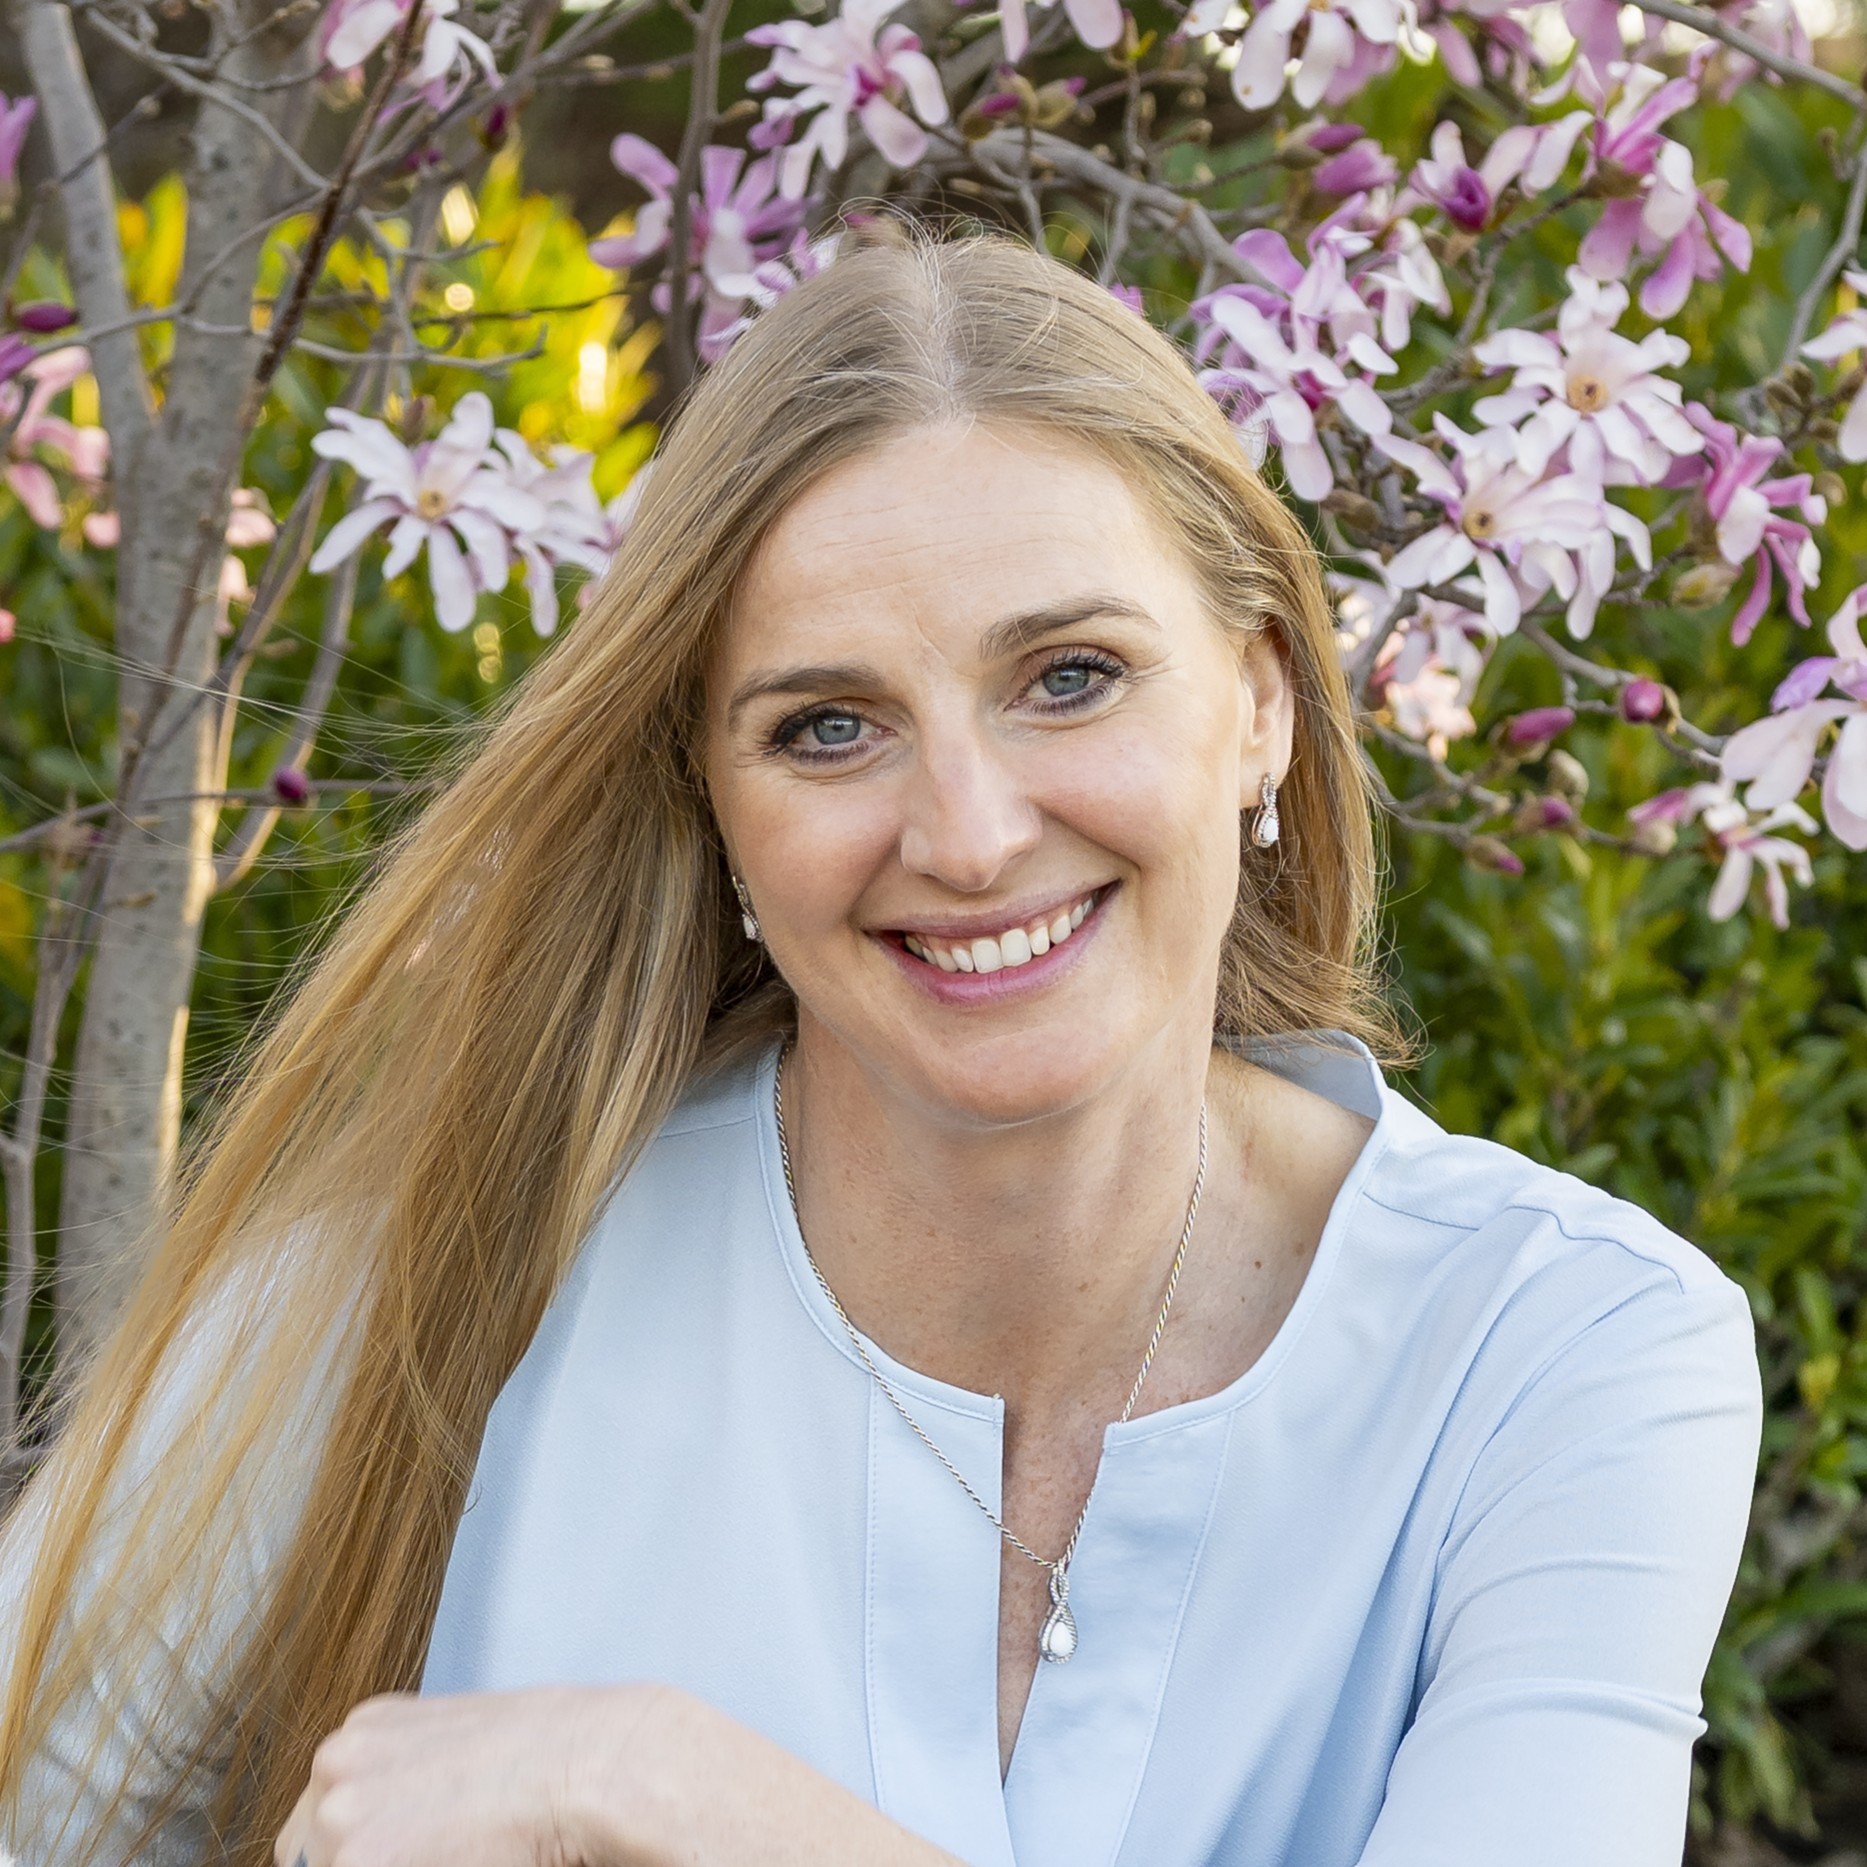
\includegraphics[width=0.25\linewidth]{../images/DSC_0624_sqre} \end{center}

Email:
\textbf{\href{mailto:lorrainegaudio@boisestate.edu}{\nolinkurl{lorrainegaudio@boisestate.edu}}}
(You can call me ``Professor Gaudio'' or ``Lorraine'' is fine too!)

Virtual Office Hours: By appointment; please email to arrange a time.

Office Location: I do not have an office this semester

Contact instructions: For the quickest response, I prefer that you
contact me by email. I respond to emails within 24 hours, except on
weekends and holidays (I may respond on weekends and holidays, but there
is no guarantee).

\chapter{Course Informaiton}\label{course-informaiton}

\section{Course Format}\label{course-format}

We will follow Canvas modules. Video lessons will be available in these
modules. You will follow along, completing practice problems in R Studio
(less than 1 hr per week). Videos and their accompanying assignments are
due before each class. Then, we will meet on Mondays to work through
additional practice problems associated with what was covered in the
video lessons. You will complete assignments in RStudio and then upload
them to Canvas. There will be plenty of time to work on the signature
assignment during our in-person class.

\section{Prerequisites}\label{prerequisites}

None other than a basic understanding of how to operate and navigate a
computer (especially the file system), the ability to download and
upload files with Canvas, and a sense of integrity (especially the
academic kind).

\section{Main Course Learning
Objectives}\label{main-course-learning-objectives}

A student successfully completing this course will be able to:

\begin{enumerate}
\def\labelenumi{\arabic{enumi}.}
\item
  Navigate the R statistical language and programming environment
\item
  Identify R Studio functions and programming concepts.
\item
  Discover the packages and code needed to conduct fundamental
  mathematical and statistical analysis in R
\item
  Write code in R to solve sample problems
\item
  Explain the importance of an open-access software environment for
  accessibility, transparency, and reproducible social science.
\end{enumerate}

\section{Additional Learning
Objectives}\label{additional-learning-objectives}

The rapid proliferation of artificial intelligence (AI) across all
aspects of life is posing challenges to education systems aimed at
preparing students. Given the transformative potential of AI for human
societies, it is crucial to equip students with the values, knowledge
and skills needed to navigate the future with AI. AI has an impact on
student learning. This course is designed to give you the skills and
foundation to be successful in an R statistics course, yet AI is highly
proficient at producing code. As a researcher, you will not only need to
precisely create new knowledge but also be able to explain it.
Additionally, using generative AI to produce R code for you will not
facilitate your learning. Yet at the same time, using generative AI to
explore R code will also accelerate your learning. This course will help
students strengthen their epistemic values while also targeting the
development of several \textbf{AI competencies}, including:

\begin{enumerate}
\def\labelenumi{\arabic{enumi}.}
\item
  \textbf{Human-centered mindset}: The dynamics of humans controlling AI
  versus AI controlling humans.
\item
  \textbf{AI techniques and applications}: Whether or not to use a
  specific AI system to achieve a justified aim. Before using AI, ask:
\end{enumerate}

\begin{itemize}
\item
  Should AI be used in a particular situation?
\item
  Which AI tool to select for a given purpose or task?
\item
  What are the boundaries, goals, and constraints of a problem?
\end{itemize}

\begin{enumerate}
\def\labelenumi{\arabic{enumi}.}
\setcounter{enumi}{2}
\tightlist
\item
  \textbf{Ethics of AI}: Transparency of use and guidelines for
  utilizing AI within rules and regulations, and privacy risks of
  certain AI systems.
\end{enumerate}

\pagebreak

The epistemic values of this course are associated with intellectual
virtues or ``\textbf{learning skills}.''

\begingroup\fontsize{9}{11}\selectfont

\begin{longtable}[t]{>{\raggedright\arraybackslash}p{3cm}>{\raggedright\arraybackslash}p{5.5cm}>{}p{7.5cm}}
\toprule
Skill & Meaning\\
\midrule
\endfirsthead
\multicolumn{2}{@{}l}{\textit{(continued)}}\\
\toprule
Skill & Meaning\\
\midrule
\endhead

\endfoot
\bottomrule
\endlastfoot
Curiosity & Asking new, relevant questions and investigating them beyond what’s assigned.\\
Autonomy & Taking initiative and making choices about your learning path, rather than waiting for exact instructions.\\
Thoroughness & Clearly documenting your steps and reasoning so someone else can follow your process.\\
Open-mindedness & Considering and testing alternative methods or perspectives, even if you already have a working answer.\\
Courage & Speaking up with ideas or questions, especially when you’re unsure, and sharing your work for feedback.\\
\addlinespace
Tenacity & Persisting through difficulties, revising code, and knowing when to seek help after genuine effort.\\
Transparency & Disclosing methods, materials, assumptions, values, and interests.\\*
\end{longtable}
\endgroup{}

\chapter{Course Requirements}\label{course-requirements}

\section{Course Materials}\label{course-materials}

All required materials will be supplied and available to download via
Canvas. The following FREE resources are recommended but \emph{not
required}. They will help you learn R programming and data analysis
concepts more effectively:

\begin{itemize}
\item
  \textbf{Introduction to Data Science} by Rafael Irizarry
  \url{https://rafalab.dfci.harvard.edu/dsbook-part-1/}. This book
  provides a comprehensive introduction to data science concepts and R
  programming.
\item
  \textbf{R for Data Science} by Hadley Wickham, Mine Çetinkaya-Rundel,
  and Garrett Grolemund \url{https://r4ds.hadley.nz/}. This book
  provides a gentle introduction to programming concepts and R.
\item
  \textbf{bookdown: Authoring Books and Technical Documents with R
  Markdown} by Yihui Xie
  {[}\url{https://bookdown.org/yihui/bookdown/}{]}\url{https://bookdown.org/yihui/bookdown/}).
  This book provides a comprehensive guide to using R Markdown for
  technical writing and documentation.
\end{itemize}

\section{Class Participation}\label{class-participation}

You will be doing coding in class with your peers. You need to be
prepared by watching the video(s) and completing the assignment(s) ahead
of time. This is because you will apply video content to additional
problems and explore beyond what is demonstrated using your selected
dataset. The instructor will be there to help you through the material.
Learning to code is a trial-and-error process.

\section{Study Time Required}\label{study-time-required}

Expect to spend approximately one hour outside of class time per week
reviewing video(s) and preparing for class. Please be aware that time
estimates for each lesson and assignment are estimates only. The actual
time you spend completing the course activities will vary depending on
how quickly you read and the level of your technology skills. On
average, students will need to spend more time preparing for class in
the second half of the semester. Organize your time in a way that allows
you to thoughtfully and thoroughly complete assignments.

\section{Grading Information}\label{grading-information}

In this course, your grade starts at zero and grows as you earn points
by showing what you can do---not by avoiding mistakes. You will never
``lose'' points because something went wrong. Instead, every activity is
a chance to build your total toward 100 points. On assignment, half of
your points will come from solving R problems (technical skills) and
half from demonstrating learning skills. These habits, like curiosity,
tenacity, and thoroughness, make you a stronger, more independent
learner. I will model these skills in lectures and videos, and you will
have many ways to show them in your work and class. The goal is for you
to leave this course not only knowing R basics, but also knowing how to
keep learning R (and other tools) long after the semester ends. Grades
in this course are based on a 100-point grading system utilizing the
allocation of points shown below.

\begin{table}[!h]
\centering\begingroup\fontsize{9}{11}\selectfont

\begin{tabular}[t]{>{\raggedright\arraybackslash}p{4.2cm}>{\centering\arraybackslash}p{1.2cm}>{\raggedright\arraybackslash}p{10.5cm}}
\toprule
\textbf{Graded Activity} & \textbf{Points} & \textbf{Description}\\
\midrule
Document Technical Skill Practice & 40 & 14 self-guided problem-solving tasks linked to the video lectures. Each is worth 2.50 points. Highest points = correct answer with working code. Partial points = partially correct or code with minor errors. Attempted but incorrect = lower partial points. No submission = 0 points. Assignments have multiple opportunities to earn points.\\
Document Learning with Memos & 40 & Short written reflections throughout your assignments that document your thought process, problem-solving steps, and use of targeted learning skills (Curiosity, Autonomy, Thoroughness, Open-mindedness, Courage, Tenacity, Transparency). Points are additive—you only gain points here, never lose them. Each memo can earn up to 0.5 points based on evidence of skill use.\\
Signature Assignment & 20 & An independent project where you get to select a real dataset to play with. You will apply R packages/functions from the course and produce a reproducible report. Your submission will include: 1) clean, runnable code, 2) explanatory comments, and 3) memos throughout.\\
\textbf{Total} & \textbf{100} & \textbf{}\\
\bottomrule
\end{tabular}
\endgroup{}
\end{table}

Tip: Confirm an assignment has been submitted and view all of your
scores and accompanying comments on graded assignments by accessing ``My
Grades'' in the Canvas course menu.

\section{Final Letter Grades}\label{final-letter-grades}

Final Letter Grades will be based on the following scale:

\begin{table}[!h]
\centering\begingroup\fontsize{9}{11}\selectfont

\begin{tabular}[t]{>{\raggedright\arraybackslash}p{3.0cm}>{\raggedright\arraybackslash}p{3.5cm}>{\raggedright\arraybackslash}p{3.5cm}>{\raggedright\arraybackslash}p{3.5cm}}
\toprule
\textbf{Grade band} & \textbf{Plus} & \textbf{Base} & \textbf{Minus}\\
\midrule
A grades & 100–98\%: A+ & 97.5–93\%: A & 92.5–90\%: A-\\
\cmidrule{1-4}
B grades & 89.5–88\%: B+ & 87.5–83\%: B & 82.5–80\%: B-\\
\cmidrule{1-4}
C grades & 79.5–78\%: C+ & 78–73\%: C & 72–70\%: C-\\
\cmidrule{1-4}
D grades & 69.5–68\%: D+ & 67.5–63\%: D & 62.5–60\%: D-\\
\cmidrule{1-4}
F grades & 59.5–0\%: F &  & \\
\bottomrule
\end{tabular}
\endgroup{}
\end{table}

\section{Late Work Policy}\label{late-work-policy}

It is always best to submit work on time, but I understand that
sometimes extenuating circumstances make this difficult. My policy on
late work is as follows: Everyone takes R at their own pace. The due
dates are guidelines more than anything. Unfortunately, it is not
possible to consider assignments turned in after \textbf{December 12th}.
If you

\chapter{Student
Expectations/Responsibilities}\label{student-expectationsresponsibilities}

\section{Communication}\label{communication}

Contact the instructor, Professor Gaudio, by email at
\textbf{\href{mailto:lorrainegaudio@boisestate.edu}{\nolinkurl{lorrainegaudio@boisestate.edu}}}
to ask questions, give status reports, or request 1:1 assistance, if
needed. You are encouraged to ask questions directly and immediately.
I'd be happy to schedule an in-person or online Zoom session to help you
out with any problem, big or small. \textbf{Every student in this course
can and should be successful.} If you need help, please reach out.

If you notice any problems in the course or seek clarification on an
assignment, send me an email or a Canvas Message. If you need technical
assistance, please call the Help Desk. For assistance with technical
problems in Canvas, please contact the Boise State Help Desk,
\textbf{\href{mailto:helpdesk@boisestate.edu}{\nolinkurl{helpdesk@boisestate.edu}}},
tel. 208-426-4357, or see
\url{https://www.boisestate.edu/oit-learning/canvas/} and scroll to the
Canvas for Students section.

\section{Student Well-Being}\label{student-well-being}

If you are struggling for any reason (COVID, relationship, family, or
life's stresses) and believe these may impact your performance in the
course, we encourage you to contact the Dean of Students at (208)
426-1527 or email
\textbf{\href{mailto:deanofstudents@boisestate.edu}{\nolinkurl{deanofstudents@boisestate.edu}}}
for support. Additionally, if you are comfortable doing so, please reach
out to me and I will provide any resources or accommodations that I can.
If you notice a significant change in your mood, sleep, feelings of
hopelessness or a lack of self-worth, consider connecting immediately
with Counseling Services (1529 Belmont Street, Norco Building) at (208)
426-1459 or email
\textbf{\href{mailto:healthservices@boisestate.edu}{\nolinkurl{healthservices@boisestate.edu}}}*.

\section{Academic Integrity}\label{academic-integrity}

Academic Integrity: a set of positive values and an agreement with
ethical and professional principles, standards, and practices that
involve the whole institution. Honesty, trust, fairness, respect,
responsibility, and courage (to name a few)

Boise State promotes Academic Excellence as a core Shared Value,
upholding the virtue of honesty in the pursuit of knowledge. Behaving
with integrity and honesty is a hallmark of a Boise State University
graduate. The conferring of a degree represents the University's
indication that the recipient has engaged in academic work that is
representative of her/his own efforts and completed with integrity and
honesty.

Upholding academic integrity in all assignments allows students to
engage with the material being investigated and assert their
evidence-based findings. This behavior demonstrates the commitment to
learning and preparation necessary for a successful future. All work you
submit must represent your own ideas and effort or be cited, including
any material you wrote for another course; when work does not, it is
academic dishonesty. Academic dishonesty in any form may result in
failure in the course or dismissal from the Program and/or the
University. See Boise State's
\href{https://www.boisestate.edu/registrar/general-information-and-policies/academic-integrity/}{Academic
Integrity} page for specific behaviors to avoid.

\section{Student AI Use}\label{student-ai-use}

Assignments will explicitly say if and which generative AI (GAI) are
allowed and how you are allowed to use them. In this course, you are
allowed to use \href{https://boisestate.ai}{boisestate.ai} to help you
troubleshoot error messages or support your curiosities. You must not
use any AI tool to directly answer your assignment questions for you.
Doing so will be a disservice to yourself, as you will not be prepared
for subsequent courses. Additionally, this will breach our agreement as
outlined in this syllabus and constitute a violation of academic
integrity. All code should by physically typed in by you and not copied
and pasted from an AI tool or other source.

An essential part of learning and discovery is embracing its challenges.
You're not likely to learn effectively if a task isn't pushing you out
of your comfort zone. GAI tools can make work easier, which is great!
However, grit (tenacity) will help you learn. Additionally, there is a
risk of over-reliance, preventing you from remaining in control of your
work. It is important to avoid skipping steps in the learning and
creative process because each step contributes to a deeper understanding
of the subject matter. AI should enhance your work, aid your curiosity,
and not replace your unique contributions. To ensure generative AI does
not blunt or prevent types of insights that you might only achieve
through independent effort, you will define an AI-human effort use for
your learning and research along with a reflection of how you feel this
use case affected your learning. This model would clarify which research
stages and processes can lean on AI automation, which need interactive
AI tool use, and when the researcher must engage in deeper thought and
reflection.

You will be transparent about when and how generative AI in your memos.
Include:

\begin{enumerate}
\def\labelenumi{\arabic{enumi}.}
\item
  A record of prompt and chat activity.
\item
  A reflection on how GAI might have aided or hindered learning or
  knowledge creation.
\end{enumerate}

\chapter{Instructor
Expectations/Responsibilities}\label{instructor-expectationsresponsibilities}

\section{Instructor AI Use}\label{instructor-ai-use}

\begin{enumerate}
\def\labelenumi{\arabic{enumi}.}
\tightlist
\item
  I may use GAI to aid in providing custom and personal feedback on your
  assignments. Your work is never uploaded into any AI tool. You may
  choose to opt out when submitting your assignment.
\end{enumerate}

\begin{itemize}
\tightlist
\item
  Question: Will the AI tool replace instructor grading?
\end{itemize}

Short Answer: No.~I will never upload your work into an AI tool.
Instead, I will use AI to improve on explaining.

\begin{itemize}
\tightlist
\item
  Question: Does opting out affect my grade?
\end{itemize}

Short Answer: No.~Both submission routes are graded with the same
rubric.

\begin{enumerate}
\def\labelenumi{\arabic{enumi}.}
\setcounter{enumi}{1}
\tightlist
\item
  I use GAI to aid in editing lessons and assignments. I am redesigning
  this course, and I am using AI to assist me in making improvements.
\end{enumerate}

\chapter{Additonal Syllabus Policies}\label{additonal-syllabus-policies}

Please refer to these documents for more information about
\href{https://docs.google.com/document/d/14ZMRsHAgo356h0nHtJuStDKGwvg6LY-XOA7PxacwECw/edit?usp=sharing}{University
Guidelines and Policies}, and
\href{https://docs.google.com/document/d/1tO-RnUbkFoQTNhFLzo7HXers2p_3OS4NUFdowagugNw/edit?usp=sharing}{Student
Expectations and Guidelines}.

  \bibliography{references.bib}

\end{document}
